\chapter{使用教程}

这里简单介绍一下模板的使用,语法部分可以对照相应的 tex 文件以及生成的 pdf 效果来进行参考。

可以对 scutthesis.cls 进行修改,进行定制化配置。

\section{文件说明}

\begin{table}[H]
    \centering
    \zihao{5}
    \caption{主要文件说明}
    \label{tab:file-description}
    %\begin{table}[]
\begin{tabular}{@{}cc@{}}
\toprule
文件/目录      & 说明           \\ \midrule
algo/          & 伪代码          \\
code/          & 代码           \\
content/       & 各章节的内容       \\
img/           & 图片           \\
table/         & 表格           \\
main.tex       & 入口文件         \\
ref.bib        & 参考文献的 bib 文件 \\
scutthesis.cls & 模板           \\ \bottomrule
\end{tabular}
%\end{table}
\end{table}

\section{表}

\LaTeX 的表格语法比较复杂,可以使用某些可视化工具,如 \href{https://www.tablesgenerator.com/}{Table Generator},在线生成 \LaTeX 表格代码后,粘帖到 tex 文件。

\autoref{tab:test} 是一个简单的表格示例。

\begin{table}[H]
    \centering
    \zihao{5}
    \caption{一个简单的表格}
    \label{tab:test}
    
\begin{tabular}{c|c|c}
\hline
      & 算法 1 & 算法 2 \\ \hline
数据集 1 &      &      \\ \hline
数据集 2 &      &      \\ \hline
\end{tabular}

\end{table}

\section{图}

封面的 logo 图如 \autoref{fig:logo} 所示。

\begin{figure}[H]
    \centering
    \caption{封面的 logo}
    \label{fig:logo}
    
\includegraphics[width=0.4\textwidth]{img/logo.png}
\end{figure}

子图的排版使用的是 \href{https://www.ctan.org/pkg/subfig}{subfig} 宏包,如 \autoref{fig:subfigure-a} 是 \autoref{fig:subfigure} 中的一个子图。

\begin{figure}[H]
    \centering
    \subfloat[子图 a\label{fig:subfigure-a}]{
        
\includegraphics[width=0.2\textwidth]{img/logo.png}
    }
    \subfloat[子图 b\label{fig:subfigure-b}]{
        
\includegraphics[width=0.2\textwidth]{img/logo.png}
    }
    \subfloat[子图 c\label{fig:subfigure-c}]{
        
\includegraphics[width=0.2\textwidth]{img/logo.png}
    }
    \\
    \subfloat[子图 d\label{fig:subfigure-d}]{
        
\includegraphics[width=0.2\textwidth]{img/logo.png}
    }
    \subfloat[子图 e\label{fig:subfigure-e}]{
        
\includegraphics[width=0.2\textwidth]{img/logo.png}
    }
    \subfloat[子图 f\label{fig:subfigure-f}]{
        
\includegraphics[width=0.2\textwidth]{img/logo.png}
    }
    \caption{多个图}
    \label{fig:subfigure}
\end{figure}

图片的绘制工具:

\begin{itemize}
    \item 如果是数据统计图,可以使用 Python / Matlab 等工具绘制并保存为 pdf / eps 格式(矢量图)。
    \item 对于简单的结构图,可以使用 \href{https://www.diagrams.net/}{draw.io} 这种绘图工具。
    绘制完,全选,导入保存为 pdf,记得把绘图信息内嵌进去(如\autoref{fig:drawio-export}),方便下次编辑图片。
\end{itemize}

\begin{figure}[H]
    \centering
    \caption{Draw.io 导出设置}
    \label{fig:drawio-export}
    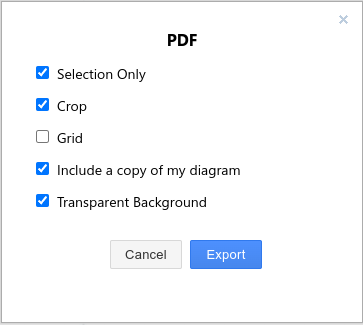
\includegraphics[width=0.3\textwidth]{img/drawio-export.png}
\end{figure}

\section{算法}

\subsection{伪代码}

伪代码部分,使用了 \href{https://ctan.org/pkg/algorithms/}{algorithm} 和 \href{https://www.ctan.org/pkg/context-algorithmic}{algorithmic} 两个宏包,伪代码的效果如 \autoref{algo:test} 所示。

关于各种伪代码宏包的区别,可以参阅 \href{https://zhuanlan.zhihu.com/p/145195565}{Latex 算法怎么写?(一):algorithm, algorithmic算法包到底什么区别?}

\begin{algorithm}[H]
    \centering
    \caption{伪代码示例}
    \label{algo:test}
    \begin{algorithmic}[1]
    \REQUIRE Data $x$
    \ENSURE Label $y$
    \STATE Show condition statement;
    \IF {condition}
        \STATE Do something;
    \ENDIF
    \IF {condition}
        \STATE Do something;
    \ELSE
        \STATE Do something;
    \ENDIF
    \IF {condition 1}
        \STATE Do something;
    \ELSIF {condition 2}
        \STATE Do something;
    \ELSE
        \STATE Do something;
    \ENDIF
    \STATE Show loop statement;
    \FOR{ $i=1$ to $n$ }
        \STATE $i \leftarrow i + 1$;
        \STATE Do something;
    \ENDFOR
    \FORALL{$i=1$ to $n$}
        \STATE Do something;
    \ENDFOR
    \WHILE{$i < n$}
        \STATE Do something;
    \ENDWHILE
    \REPEAT
        \STATE Do something;
        \STATE $i \leftarrow i + 1$;
    \UNTIL{$i > n$}
    \LOOP
        \STATE Do something;
    \ENDLOOP
    \STATE Symbol: \NOT, \AND, \OR, \XOR, \FALSE, \TRUE
    \RETURN $y$
\end{algorithmic}

\end{algorithm}

\subsection{代码}

代码高亮部分使用了 \href{https://www.ctan.org/pkg/minted}{minted} 宏包,minted 主要有文件内和外部文件两种。
文件内直接在 tex 写皆可,外部文件则是由 tex 引入外部代码文件。

下面是一个文件内的 Python 代码:
\begin{minted}[]{python}
print('Hello World')
\end{minted}

如下为一段简单的 C++ 代码。
\inputminted{c++}{code/test.cpp}

\section{数学公式}

行内公式:$a_n = a_{n-1} + 1$

\autoref{eq:test} 是一个有编号公式。
\begin{equation}
    \label{eq:test}
    a_n = a_{n-1} + 1
\end{equation}

无编号公式:
$$
    a_n = a_{n-1} + 1
$$

常用的辅助工具:

\begin{itemize}
    \item \href{http://detexify.kirelabs.org/classify.html}{Detexify}:鼠标轨迹识别为 \LaTeX 符号代码。
    \item \href{https://mathpix.com/}{Mathpix}:将图片的数学公式识别为 \LaTeX 代码。
\end{itemize}

\section{数学环境}

这里使用的是 \href{https://ctan.org/pkg/amsthm} 宏包,可以参考 \href{https://zhuanlan.zhihu.com/p/133244838}{Latex 定理和证明类环境的配置(amsthm)} 进行配置。

% TODO: description
在 scutthesis.cls 可查看模板配置了哪些数学环境。

\section{化学}

这一部分使用了 \href{https://ctan.org/pkg/mhchem}{mhchem} 和 \href{https://ctan.org/pkg/chemfig}{chemfig}。

\subsection{化学式与方程式}

例子:
\begin{itemize}
    \item \ce{2H2 + O2 ->T[燃烧] 2H2O}
    \item \ce{N2 + 3H2 <=>T[高温、加压][催化剂] 2NH3}
    \item \ce{^{227}_{90}Th+}
    \item \ce{KCr(SO4)2 * 12H2O}
    \item \ce{C6H5-CHO}
    \item \ce{X=Y#Z}
\end{itemize}

\section{单位}

这一个部分使用 \href{https://ctan.org/pkg/siunitx}{siunitx} 宏包,例如 
\begin{itemize}
    \item \SI{1.5}{cm^3/min}
    \item \SI{}{\degreeCelsius}。
\end{itemize}

\section{引用}

\subsection{论文}

这部分使用了 \href{https://ctan.org/pkg/biblatex}{biblatex} 宏包,样式采用 gb7714-2015 标准。

引用有两种,上标的\upcite{he2016deep}和非上标的\parencite{he2016deep}。
有时候需要多篇引用,例如 \parencite{he2016deep, krizhevsky2012imagenet, vaswani2017attention},
根据场景决定是否采用上标形式 \upcite{he2016deep, krizhevsky2012imagenet, vaswani2017attention}。
也有这种不带方括号的,如 \supercite{he2016deep, krizhevsky2012imagenet, vaswani2017attention}。

BibTex 信息可以通过此操作获得:在 \href{https://scholar.google.com}{Google Scholar} 上面搜索相应的论文,然后点击引用,再选择 BibTex 格式(如 \autoref{fig:google-scholar-bibtex})。
把获得的文本\textbf{进行修改(根据论文要求的格式)}后,再粘帖到 ref.bib 文件中。

\begin{figure}[H]
    \centering
    \caption{Google Scholar 到处 BibTex}
    \label{fig:google-scholar-bibtex}
    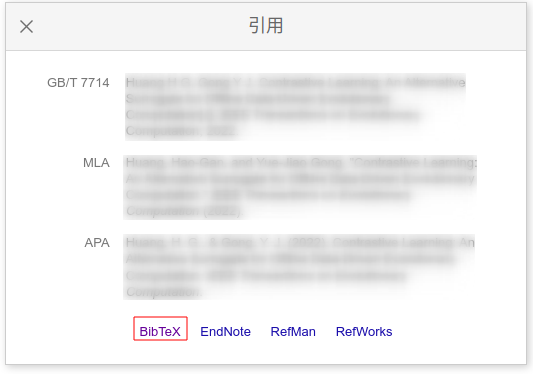
\includegraphics[width=0.5\textwidth]{img/google-scholar-bibtex.png}
\end{figure}

\subsection{图、表等}

这部分使用了 \href{https://ctan.org/pkg/hyperref}{hyperref} 宏包,

\section{脚注}

内容 \footnote{脚注内容}。
